\chapter{Design}
\label{chap:design}

This chapter explains the design process undertaken considering both the literature review research \see{chap:litrev} and the established requirements \see{chap:requirements}.
\section{Assumptions and Decisions Taken}
\label{design:assumptions/decisions}

Client discussion required assumptions and decisions to be made to assist in the project's development and progression.

A decision was made to build the artefact as a web application, providing an easily accessible pre-existing user base. Different screen sizes were accommodated with the use of CSS media queries, however, the artefact was aimed at desktop environments, with mobile support implemented in the future. 

It was assumed that the target users would have a pre-existing knowledge of route planning having used similar systems in the past. Therefore, instructions to use the artefact were not provided. Furthermore, a minimal UI was developed to ensure ease of use, whilst enabling custom route planning functionality \see{design:ui}.

Research was undertaken into different available open-source routing algorithms. OpenRouteService (ORS) (\cite{noauthor_openrouteservice_nodate}) was chosen due to its customisability and native support of round-trip route planning.

LocalStorage was used to store specific data, such as authentication tokens and last route planned. Data such as the last planned route enabled the user to load the previous route when opening the artefact after having used it previously. Other data such as authentication tokens, enabled the artefact to remain logged into external services such as Strava (\cite{noauthor_strava_nodate}), Garmin Connect (\cite{international_garmin_nodate}) and Google Drive (\cite{noauthor_home_nodate}).

\section{User Interface}
\label{design:ui}
Initially, hand-drawn low-fidelity prototypes were created for two iterations of the artefact \see{fig:lofi1}, demonstrating some design changes in the second low-fidelity prototype \see{fig:lofi2}. After the low-fidelity prototypes were complete, a high-fidelity prototype was created based on the second design using MarvelApp (\cite{noauthor_marvel_nodate}).

The following components form the overall User Interface (UI): Map,  ElevationChart, Router, RoutePreferencesPanel and the Weather/LeftPanel. The primary root component which other components depended on was the Map component; with other components adding enhanced functionality to the artefact.

\subsection{Colour Scheme}
\label{ui:colourscheme}

The plain colour scheme was chosen for simplicity and ease of use of the artefact. Dark mode was chosen against after researching pre-existing route planners, it was found that a light map, and surrounding UI was generally considered more usable to the average user. A dark mode could be implemented in the future, enabling the user to switch modes should they choose.

\subsection{Low Fidelity Prototype}
\label{ui:low-fi}

Low-fidelity prototyping was vital in the project's early stages, ensuring that all UI elements would meet the user expectations and requirements. With the project's focus on enhanced routing features, it was critical to ensure that the designs were simple, maximising usability, whilst still including all the required functionality. Two iterations were divided into two separate low-fidelity prototypes, where the first demonstrates the core functionality \see{fig:lofi1}, whereas the second also includes some extended functionality \see{fig:lofi2}.

\subsection{High-Fidelity Prototype}
\label{ui:hi-fi}

The high-fidelity prototype was made after low-fidelity prototyping had concluded. The second low-fidelity prototype was expanded upon at this stage. It was critical to ensure the high-fidelity prototype wouldn't overbear the user with too much information at once, therefore the necessary functionality was available in the main view \see{fig:hifi1}, whereas extra options are hidden behind dropdown menus \see{fig:hifi2}.

  \begin{figure}[!ht]
    \centering
    \includegraphics[width=350px]{figures/lofi-1.png}
    \caption{Low-Fidelity Prototype 1}
    \label{fig:lofi1}
  \end{figure}

  \begin{figure}[!ht]
    \centering
    \includegraphics[width=350px]{figures/lofi-2.png}
    \caption{Low-Fidelity Prototype 2}
    \label{fig:lofi2}
  \end{figure}

  \begin{figure}[!ht]
    \centering
    \includegraphics[width=400px]{figures/hifi-1.png}
    \caption{High-Fidelity Prototype 1}
    \label{fig:hifi1}
  \end{figure}

  \begin{figure}[!ht]
    \centering
    \includegraphics[width=400px]{figures/hifi-2.png}
    \caption{High-Fidelity Prototype 2}
    \label{fig:hifi2}
  \end{figure}

  \clearpage
\section{Use Cases}
\label{design:usecase}
Use cases were determined by discerning potential uses of the artefact, subsequently, a use case diagram was then created to visualise these cases. The diagram is formed of actors, tasks and system components that are required when each task is performed. Visual Paradigm was used to create the use case diagram (\cite{noauthor_ideal_nodate}).

\subsection{Use Case Diagram}
\label{usecase:diagram}
The target user groups were identified during requirements gathering. Users were grouped into a single actor because each user group would access identical functionality \see{chap:requirements}. Therefore, all users can access all functionalities, where they can use the extended features as they require \see{fig:usecase}.

\begin{figure}[!ht]
  \centering
  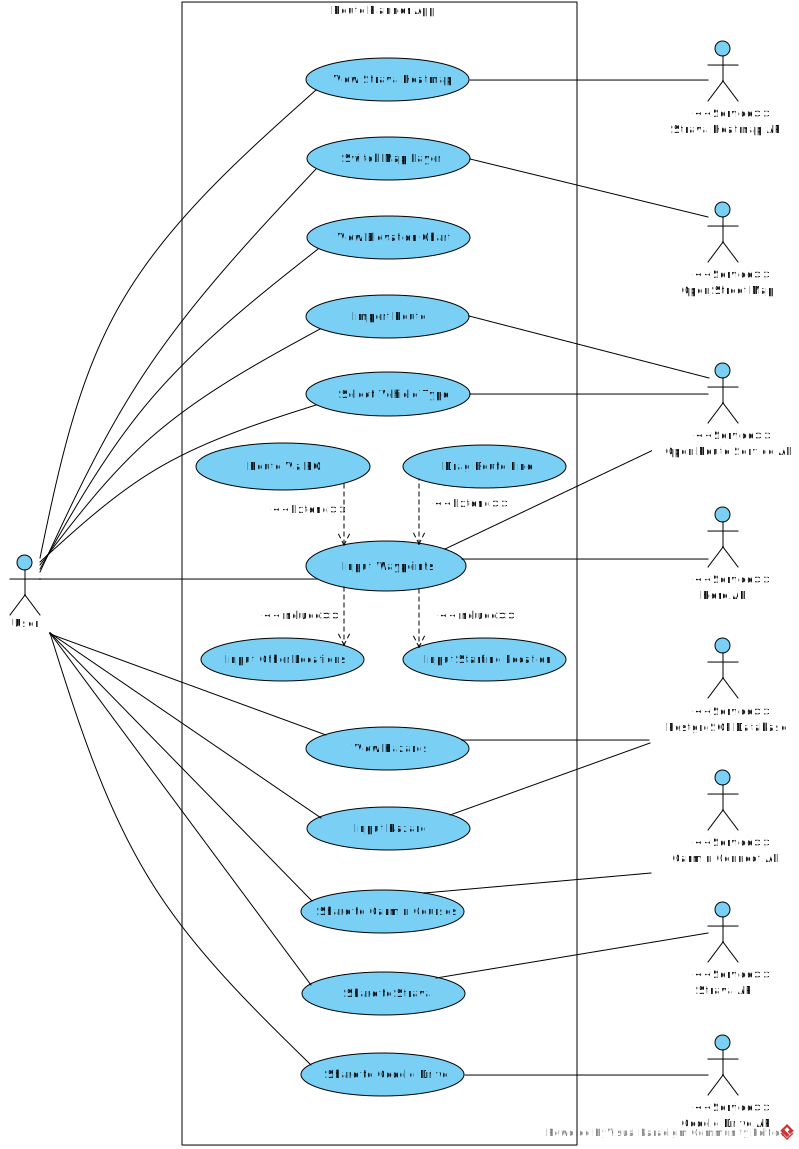
\includegraphics[width=400px]{figures/use-case.png}
  \caption{Use Case Diagram}
  \label{fig:usecase}
\end{figure}

\section{System Design}
\label{design:system}

It is vital to also design the back-end system. The back-end is comprised of the Go/Gin Web Server, PostgreSQL (PSQL) database and the React client. This section delves further into the internal design of the artefact. 

\subsection{Architecture Design}
\label{system:architecture-design}

The client-server architecture was used to build the artefact \see{fig:clientserver}. This architecture was selected to enable easy expansion of the artefact, aiming to host the web application centrally, along with the PSQL database \see{system:database-design}. This architecture was critical for security reasons to use different services requiring oauth, which enforce authentication through the server. Furthermore, this architecture enabled different processes to be handled via the server, reducing the overall load the client application requires to run.

Client-server architectures do add the risk of a single point of failure, whereby the application is wholly dependant on the web server. Overall the risk was deemed minimal because sensitive information isn't stored \see{tab:risk-assessment}. In the case of a system failure, the application would remain inaccessible until fixed, however, thorough testing has been undertaken to reduce the risk \see{chap:testing}.

\clearpage
\begin{figure}[!ht]
  \centering
  \includegraphics[width=250px]{figures/client-server.png}
  \caption{Client-Server Architecture}
  \label{fig:clientserver}
\end{figure}

\subsection{Database Design}
\label{system:database-design}

The database crucial in extending the artefacts functionality, it servers as a hazard index database, whilst also storing hazardous cycling infrastructure. PSQL was chosen as the Relational Database Management System (RDBMS), as PostGIS was available to use to add the functionality for storing, indexing and querying geospatial data (\cite{noauthor_postgis_nodate}). This is used to display hazard areas on the map that users should avoid, with the potential to include native routing support to avoid these hazards, further highlighted under future work \see{evaluation:future} \see{fig:erd}. 

\begin{figure}[!ht]
  \centering
  \includegraphics[width=350px]{figures/erd.png}
  \caption{Entity Relationship Diagram}
  \label{fig:erd}
\end{figure}

\subsection{Modular Architecture}
\label{system:modular-architecture}
React.js provides a modular design approach with components where variables are stored in the form of state which can re-render the application where necessary. All necessary data, functions and states can be passed to and from different components using the built-in props functionality, where components have a parent-child relationship \see{fig:components}.

While the App.jsx file is the starting point of the React application, the Map component acts as the primary parent for most of the artefact's components. Multiple states and variables are declared within Map and are transferred across the rest of its children. This setup is necessary because most components are dependent on the Map to function. However, not all child components of Map are required for the application to function, demonstrating the modular functionality of the application. The LeftPanel component and its children remain standalone from the rest of the application as these components act to display information on load.

\begin{figure}[!ht]
  \centering
  \includegraphics[width=400px]{figures/components.pdf}
  \caption{Modular Components}
  \label{fig:components}
\end{figure}

\clearpage 
\section{Critique of Designs}
\label{design:critique}

The progressive approach was used to develop the UI, and whilst beneficial to the overall project and its aims, mobile devices were not catered for. While this can be seen as bad practice, the artefact is aimed at users on a desktop environment, exporting routes to external mobile navigation/fitness applications. Therefore, a mobile-first design was not opted for.

Both high-fidelity designs \see{ui:hi-fi} only demonstrate a light colour scheme. Due to this, all users are forced to use the light mode with no option to customise. In hindsight, it would have been beneficial to develop multiple high-fidelity designs to include both a light and dark mode.

The database was designed to store hazard and cycling infrastructure information \see{system:database-design}, ideally, the database would store more than just this data. To expand some of the artefact's basic functionality, the database would also store user oAuth tokens, as well as their planned routes. Implementing such tables would enable the user to save and load routes to the their accounts on the artefact without the requirement to store GPX/GeoJSON files locally \see{evaluation:future}. These tables would also enable a more expansive sharing functionality to social media, enabling users to share links to routes, rather than map screenshots of their routes.

Finally, the modular architecture approach \see{system:modular-architecture}, was ideal for developing the artefact, however, the modules could have been better structured to maximise the benefits of this approach. The artefact should be customisable, whereby modules can be disabled entirely if they are not required. At this stage, the design only caters to the manual disabling of each module, with certain modules being necessary for the artefact to function.

\section{Conclusion}
\label{design:conclusion}

Overall, the design process proved critical, ensuring that the artefact met all the requirements \see{chap:requirements} and objectives \see{intro:aimsandobjectives}. The designs were followed closely during iterations 2 and 3 \see{chap:implementation}, however, iteration 1 \see{implementation:iteration1} was developed before these were complete. The following chapter will delve into the implementation of the artefact, demonstrating how the design decisions made were integrated into the final product.
